
\chapter{Introduction}

In the early days of the artificial intelligence, the field rapidly tackled  and solved problems that are intellectually difficult for human beings but realtively straightforward for computers -- problems that can be described by a list of formal, mathematical rules.
The true challenge to artificial intelligence proved to be solving the tasks that are easy for every people to perform but hard for people to describe formally -- problems that we solve intuitively, but feel automatic, like recognizing spoken words or faces in images.


The solution is to allow computers to learn from experience and understand the world in terms of a hierarchy of concepts, with each concept defined through its relation to simpler concepts.
By gathering knowledge from experience, this approach avoids the need for human operators to formally specify all the knowledge that the computer needs.
The hiearachy of concepts enables the computer to learn complicated concepts by building them out of simpler ones.
If we draw a graph showing how these concepts are built on top of the each other, the graph is deep, with many layers.
For this reason, we call this approach to AI \keywords{deep learning}.


The first artificial intelligence projects are called the \keywords{knowledge base}.
Knowledge about the world is hard-coded in a formal languages.
A computer can reason automatically about statements in these formal languages using logical inference rules.
However none of these project has led to a major success.


The difficulty faced by systems relying on hard-coded knowledge suggest that AI systems need the ability to acquire their own knowledge, by extracting patterns from raw data. This capability is known as \keywords{machine learning}. 

However, the performance of machine learning algorithms depends heavily on the \keywords{representation} of the data.
Each piece of information included in the representation is known as a \keywords{feature}.


For many tasks, however, it is difficult to know what features should be extracted. One solution to this problem is to use machine learning to discover not only the mapping from representation to output but also the representation itself. This approach is known as \keywords{representation learning}.



Of course, it can be very difficult to extract high-level, abstract features from raw data.
When it is nearly difficult to obtain a representation as to solve the original problem, representation learning does not seem to help us.


\keywords{Deep learing} solves this central problem in representaion learing by introducing representaions that are expressed in terms of other, simpler representaions.


The evolution of deep learning is show in Figure \ref{fig:evolution-of-deep-learning}:
\begin{figure}[!ht]
  \centering
  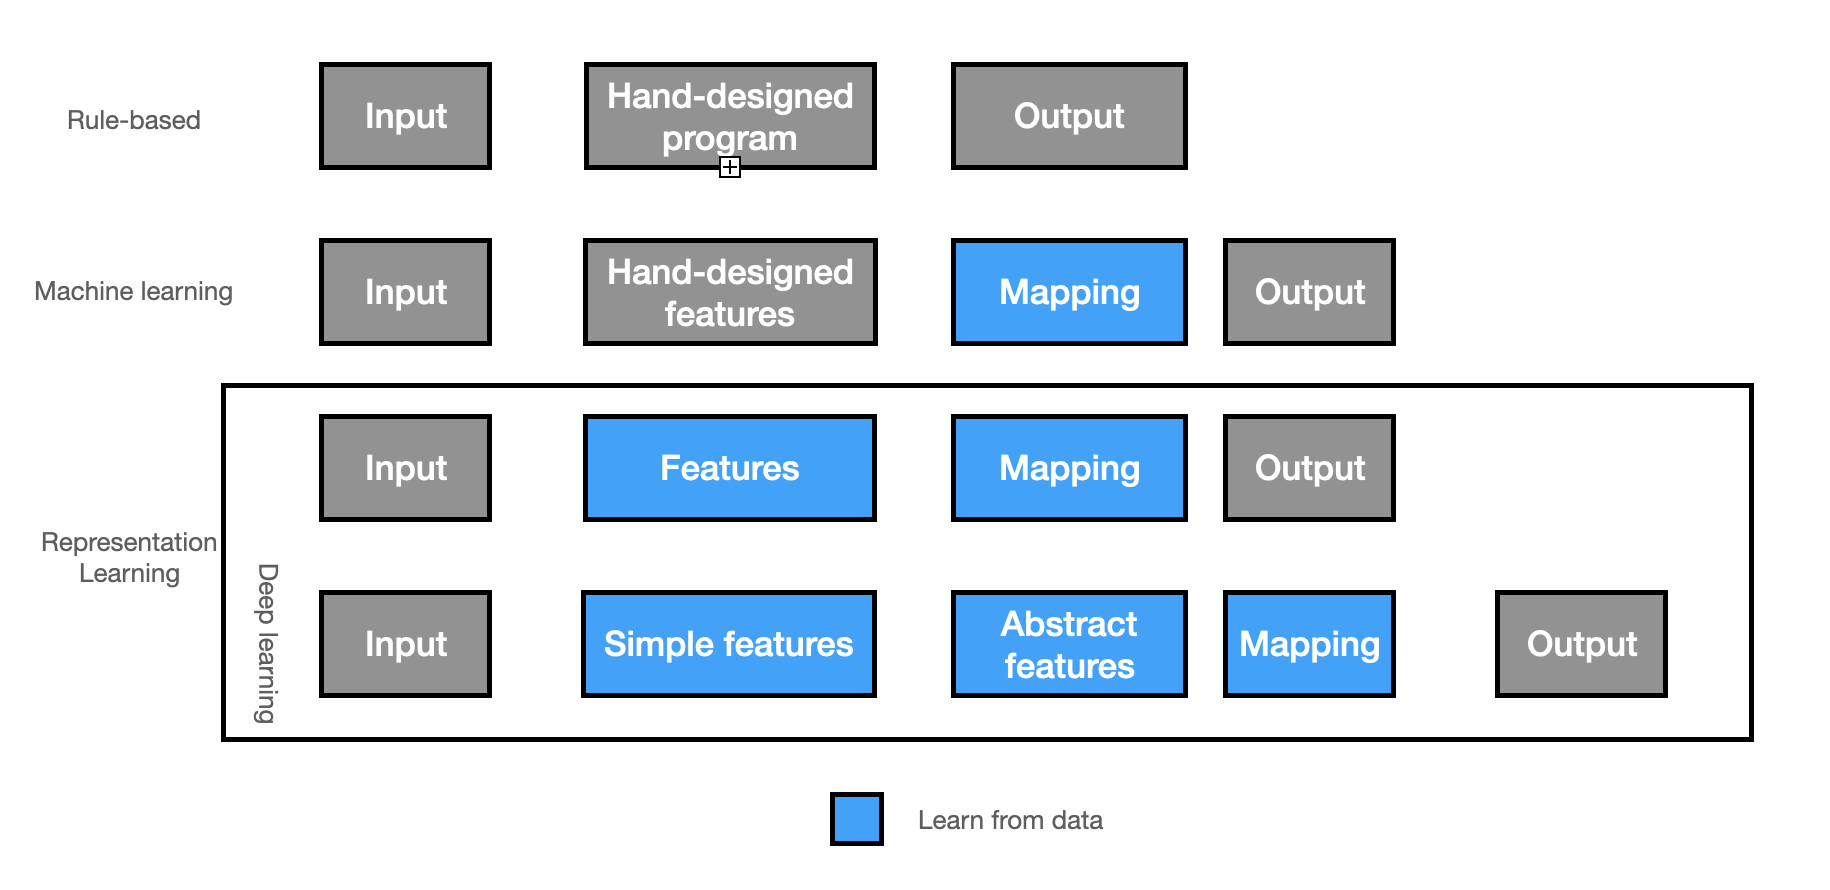
\includegraphics[width=\textwidth]{evolution-of-deep-learning.png}
  \caption{Evolution of deep learning}
  \label{fig:evolution-of-deep-learning}
\end{figure}